\documentclass[11pt,a4paper,oldfontcommands,openany]{memoir}
\usepackage[utf8]{inputenc}
\usepackage[T1]{fontenc}
\usepackage{microtype}
\usepackage[dvips]{graphicx}
\usepackage{xcolor}
\usepackage{times}
\usepackage{amsmath}
\usepackage{amsthm}
\usepackage{syntax}
\usepackage{multicol}

\usepackage[
breaklinks=true,colorlinks=true,
%linkcolor=blue,urlcolor=blue,citecolor=blue,% PDF VIEW
linkcolor=black,urlcolor=black,citecolor=black,% PRINT
bookmarks=true,bookmarksopenlevel=2]{hyperref}

\usepackage{geometry}
% PDF VIEW
% \geometry{total={210mm,297mm},
% left=25mm,right=25mm,%
% bindingoffset=0mm, top=25mm,bottom=25mm}
% PRINT
\geometry{total={210mm,297mm},
left=20mm,right=20mm,
bindingoffset=10mm, top=25mm,bottom=25mm} %top=25mm,bottom=25mm

\OnehalfSpacing
%\linespread{1.3}

%%% CHAPTER'S STYLE
\chapterstyle{bianchi}
%\chapterstyle{ger}
%\chapterstyle{madsen}
%\chapterstyle{ell}
%%% STYLE OF SECTIONS, SUBSECTIONS, AND SUBSUBSECTIONS
\setsecheadstyle{\Large\bfseries\sffamily\raggedright}
\setsubsecheadstyle{\large\bfseries\sffamily\raggedright}
\setsubsubsecheadstyle{\bfseries\sffamily\raggedright}


%%% STYLE OF PAGES NUMBERING
%\pagestyle{companion}\nouppercaseheads 
%\pagestyle{headings}
%\pagestyle{Ruled}
\pagestyle{plain}
\makepagestyle{plain}
\makeevenfoot{plain}{\thepage}{}{}
\makeoddfoot{plain}{}{}{\thepage}
\makeevenhead{plain}{}{}{}
\makeoddhead{plain}{}{}{}


\maxsecnumdepth{subsection} % chapters, sections, and subsections are numbered
\maxtocdepth{subsection} % chapters, sections, and subsections are in the Table of Contents

\newtheorem*{theorem}{Theorem}
\newtheorem*{definition}{Definition}
\newtheorem*{property}{Property}
\newtheorem*{lemma}{Lemma}

%%%---%%%---%%%---%%%---%%%---%%%---%%%---%%%---%%%---%%%---%%%---%%%---%%%

\begin{document}

%%%---%%%---%%%---%%%---%%%---%%%---%%%---%%%---%%%---%%%---%%%---%%%---%%%
%   TITLEPAGE
%
%   due to variety of titlepage schemes it is probably better to make titlepage manually
%
%%%---%%%---%%%---%%%---%%%---%%%---%%%---%%%---%%%---%%%---%%%---%%%---%%%
\thispagestyle{empty}

{%%%
\sffamily
\centering
\Large

~\vspace{\fill}

{\huge 
Invariant Synthesis by Counterexample Generalization
}

\vspace{2.5cm}

{\LARGE
Mickaël LAURENT
}

\vspace{3.5cm}

Carnegie Mellon University\\
Ecole Normale Supérieure Paris-Saclay

\vspace{3.5cm}

Supervisor: Bryan PARNO

\vspace{\fill}

March-July 2018

%%%
}%%%

\clearpage%\cleardoublepage
%%%---%%%---%%%---%%%---%%%---%%%---%%%---%%%---%%%---%%%---%%%---%%%---%%%
%%%---%%%---%%%---%%%---%%%---%%%---%%%---%%%---%%%---%%%---%%%---%%%---%%%

\tableofcontents*

\clearpage

%%%---%%%---%%%---%%%---%%%---%%%---%%%---%%%---%%%---%%%---%%%---%%%---%%%
%%%---%%%---%%%---%%%---%%%---%%%---%%%---%%%---%%%---%%%---%%%---%%%---%%%

\chapter{Presentation of IVy}

    \section{Context}

    As distributed programs become more and more widespread, their verification is a major challenge.

    The general purpose of my internship is to make the certification of those programs easier.
    Certifying a program consists in writing some specifications (in our case, some safety properties), and then proving than the program satisfy them.
    Several languages and tools already exist for that:

    \begin{itemize}
        \item Proof-assistants (Coq, F*, etc.):
        Powerful logics can be used for the specification,
        however the user has to manually write the proof (in a interactive way).
        \item SMT-solver based tools (dafny, F*, etc.):
        Logics and constructions are often restricted, but specifications can automatically be checked using a SMT-solver.
        Most of time, this process is undecidable,
        so there are 3 possible outputs:
        \begin{itemize}
            \item Yes, the program matches the specifications
            \item No, the program doesn't match the specifications (sometimes a counterexample can be provided)
            \item I don't know whether the program matches the specifications or not.
        \end{itemize}
        When this last case occurs, the user has to reformulate the specifications differently or to explicitely write some intermediate properties (like inductive invariants)
        in order to help the SMT-solver.
    \end{itemize}

    IVy is a language that allows the user to certify its program using a SMT-solver based approach. [REF]
    However, unlike most of its concurrents, IVy restricts the language and the logic used for specifications
    in order to be able to check the program in a decidable way.

    This approach has many advantages:
    \begin{itemize}
        \item Once the program is written and specified in an accepted logic, it can be checked more easily:
        the checker can always decide whether the program matches the invariants or not, and give a counterexample if it does not.
        \item It does not rely on any heuristic/specificity of the SMT-solver used.
        When a program cannot be checked, we always know the reason.
        \item A program can be checked with any version of any SMT-solver (because it does not depend on any heuristic).
    \end{itemize}
    
    The main disadvantage is that the user is forced to specify its program in a decidable fragment of first order logic:
    it can force him to rethink the architecture of its code, to fragment its code by creating intermediate abstract modules,
    to add some `ghost' variables, etc.

    \section{The RML language}

    IVy is inspired by a modeling language called RML (Relational Modeling Language). It is restricted such that some decidability properties are guaranteed (see section 1.4).
    A RML program is composed of:
    \begin{itemize}
        \item Some uninterpreted types that we call `sorts' (uninterpreted means that they are not constrained by any existing theory like arithmetic). A sort has an unbounded number of elements (`values').
        \item Some variables, relations and functions over these types (a variable can be considered like a function of arity 0, and a relation can be considered as a function
        which returns a boolean). These elements are mutable (their valuation can be modified by the transitions described below).
        \item Some axioms over these variables, functions and relations. Axioms are \(\exists^*\forall^*\) formulas (\( \phi_{EA} \) in the grammar below).
        \item Some transitions that we call `actions'. An action is a \(statement\) (see the grammar below).
        \item A special `init' action that is only executed once at the beginning (before any other action).
    \end{itemize}

    The transitions can be written using the following grammar:
    \begin{multicols}{2}
        \begin{grammar}

            <statement> ::= skip
            \alt abort
            \alt \textbf{r}(\(\bar{x}\)) := \( \phi_{QF}(\bar{x}) \)
            \alt \textbf{f}(\(\bar{x}\)) := \( t(\bar{x}) \)
            \alt \textbf{v} := \( * \)
            \alt assume \( \phi_{EA} \)
            \alt \( statement \) ; \( statement \)
            \alt \( statement \) | \( statement \)
            
        \end{grammar}

        \columnbreak

        \begin{grammar}

            <t> ::= \(x\)
            \alt \textbf{v}
            \alt \textbf{f}(\(t,...t\))
            \alt ite(\( \phi_{QF},t,t\))

            <\( \phi_{QF} \)> ::= \textbf{r}(\(t,\ldots t\))
            \alt \( t = t \)
            \alt \( \phi_{QF} \land \phi_{QF} \) \quad | \quad \( \phi_{QF} \lor \phi_{QF} \) \quad | \quad \( \neg \phi_{QF} \)
            
            <\( \phi_{EA} \)> ::= \( \exists x_1,\ldots,x_n \forall x_{n+1},\ldots,x_{n+m} \phi_{QF} \)

        \end{grammar}
    \end{multicols}

    The semantic of terms and formulas is as usual. The semantic of statements will be described later in the section 1.4.

    One important thing to note is that RML only allows uninterpreted sorts and booleans (and possibly other enumerated types).
    It means that types and operations over these types are only constrained by the axioms of the RML program,
    and the form of these axioms is quite restrictive.
    In particular, we can't define arithmetic operations (see section 1.3).
    However, we will see later that it is possible to extend it with linear integer arithmetic or some other theories.

    Also, unlike some other languages like F*, IVy does not allow refinement types or dependent types (for decidability reasons).
    As a consequence, we can't encode any property in the types.
    Instead, the specifications of the program will be expressed using assertions and invariants.

    \section{Decidable logics}

    In this section, we will describe the Bernays-Schönfinkel class of formulas. It is a decidable fragment of the first order logic that is used by IVy.
    We will refer to it as EPR (for Effectively Propositional) because this logic can be effectively translated into propositional logic (see the subsection 1.3.2).

        \subsection{The Bernays-Schönfinkel class (EPR)}

        The Bernays-Schönfinkel class is the set of first-order formulas such that:
        \begin{itemize}
            \item Under the prenex normal form, they have an \(\exists^*\forall^*\) quantifier prefix
            (a formula in prenex normal form is composed of a string of quantifiers called the prefix, followed by a quantifier-free part).
            \item They do not use any function symbol (only a finite number of constants and relations).
        \end{itemize}

        For instance, the following formulas define a total relation order and are in the Bernays-Schönfinkel class:
        \begin{align*}
            \forall x. \ R(x,x) &\quad\text{(reflexivity of R)}\\
            \forall x,y,z. \ R(x,y) \land R(y,z) \rightarrow R(x,z) &\quad\text{(transitivity of R)}\\
            \forall x,y. \ R(x,y) \land R(y,x) \rightarrow x=y &\quad\text{(antisymetry of R)}\\
            \forall x,y. \ R(x,y) \lor R(y,x) &\quad\text{(totality of R)}
        \end{align*}

        \subsection{Deciding the satisfiability}

        We want to decide whether an EPR formula is satisfiable or not. Let's consider for instance the following formula:
        \begin{align*}
            F: \exists x. \forall y. \ R(y,y) \land \neg R(x,y)
        \end{align*}

        This formula is not satisfiable, because for any value of \(x\), the formula \(R(y,y) \land \neg R(x,y)\) is false when we take \(y=x\).
        However, there is infinitely many possible interpretations for the relation \(R\) (because the set of possible values for \(x\) and \(y\) is not bounded).
        So how to decide the satisfiabilty of such formulas?

        First, we can get rid of the existential quantifier by introducing a new constant \(A\):
        \begin{align*}
            \forall y. \ R(y,y) \land \neg R(A,y)
        \end{align*}

        This is called the skolem normal form of \(F\).
        Note that in the general case, we can eliminate any existential quantifier in a formula in prenex normal form by introducing a new function
        that depends on all universally quantified variables in its scope. This process is called `skolemization' and preserve the satisfiability of the formula.

        \begin{property}[Skolemization]
            Let \(F\) be a formula and \(F'\) be the formula obtained after solemization if \(F\). Then \(F\) is satisfiable iff \(F'\) is satisfiable.
        \end{property}

        Now, we want to restrict the domain of the possible interpretations in order to be able to decide the satisfiability of our formula.

        \begin{definition}[Herbrand domain]
            The Herbrand domain of a formula is the set of every term that can be written with the constants and functions symbols present in the formula
            (if there is no constant symbol in the formula, we introduce a new one).
        \end{definition}

        Our formula has a unique constant \(A\) and no function symbol (only a relation symbol), so its Herbrand domain is the following:
        \( \{A\} \). More generally, we have the following property:
        
        \begin{property}
        The Herbrand domain of an EPR formula is finite.
        \end{property}

        Thus, we can decide whether or not our formula is satisfiable by an interpretation over it's Herbrand domain.
        For that, we just have to test every interpretation of \(R\) over the domain \( \{A\} \):

        \begin{itemize}
            \item With \(R(A,A)=\text{false}\): \(\forall y. \ R(y,y) \land \neg R(A,y)\) is false (with \( y \in \{A\} \))
            \item With \(R(A,A)=\text{true}\): \(\forall y. \ R(y,y) \land \neg R(A,y)\) is false (with \( y \in \{A\} \))
        \end{itemize}

        So our formula is not satisfiable by any interpretation over it's Herbrand domain.

        Finally, by applying the following theorem, we can conclude that our formula is not satisfiable by any interpretation (over any domain):
        \begin{theorem}[Herbrand]
            An universally quantified first-order formula \(F\) is satisfiable iff it is satisfied by an interpretation over it's Herbrand domain.
        \end{theorem}

        This process can be used to decide the satisfiability of any EPR formula. Moreover, when a formula is satisfiable,
        it gives us an interpretation over the Herbrand domain that satisfy the formula (= a model).
        The Herbrand domain being finite, we have the following property:

        \begin{property}[Finite model property]
            Every satisfiable EPR formula has a finite model.
        \end{property}

        \subsection{EPR with types}

        In RML, relations, functions and constants (that are preferably called `variables' since they are mutable) have types.
        For instance, a function takes arguments of some specific sorts and also return a value in a specific sort (sorts are unbounded set of values).

        We can easily add these typing constraints to the logical symbols we used in the previous subsection.
        Moreover, it allows us to extend the domain of EPR formulas by still keeping a finite Herbrand domain.

        Indeed, we can allow function symbols and \(\forall\exists\) quantifier alternation as long as,
        once the formula is skolemized, all function symbols are stratified (that is, there exists
        an order over the sorts such that, for every function symbol \( f: t_1 \to t_2 \), we have \( t_1 < t_2 \)).
        In this way, the formula will still has a finite Herbrand domain.

        However, the EPR fragment can still be too restrictive: for instance, we can't introduce linear arithmetic using only EPR axioms.
        Indeed, the standard way to define integers is to introduce a successor function symbol, which is not allowed because it is not stratified.
        More generally, we can't characterize any infinite set with only EPR axioms: it would contradict the finite model property.

        \subsection{Extensions of EPR}

        Some strict extensions of EPR are still decidable.
        In particular, SMT-solvers like Z3 [ref] are able to decide the Finite Almost Uninterpreted (FAU) fragment of first order logic,
        which add to EPR some usual interpreted symbols of Linear Arithmetic (integer constants, `+', `\( \leq \)') under some additional constraints.
        You can refer to [REF] for more details about it. 
        
        In this report, we will not use such extension of EPR, because it breaks the finite model property.
    
    \section{Checking a RML program}

    \begin{definition}[Structure \& State]
        For a given RML program, a structure is a pair \(((D_s)_{s\in \text{sorts}}, (I_s)_{s\in \text{symbols}})\) where:
        \begin{itemize}
            \item For all \(s \in \text{sorts}\), \(D_s\) is a finite domain associated to the sort \(s\).
            \item For all \(s \in \text{symbols}\) (variable, function or relation), \(I_s\) is an interpretation (=valuation) for the symbol \(s\) over the corresponding domains of \((D_s)\).
        \end{itemize}
        A state is a structure that satisfy every axiom defined in the RML program.
    \end{definition}

    In order to certify that a RML program never abort abnormally, we must provide IVy with an invariant \(I\) such that:
    \begin{enumerate}
        \item \(I\) is initially satisfied (after any execution of the `init' action from any state).
        \item \(I\) is inductive, that is: for any state satisfying \(I\), the new state of the program after executing any action of the RML program must also satisfy \(I\).
        This also implies that actions never abort abnormally from a state satisfying \(I\).
    \end{enumerate}

    To formalize these two properties, we introduce the notion of weakest precondition \(wp\):
    \begin{definition}[Weakest precondition]
        For any statement \(S\) and formula \(Q\), the weakest precondition of \(Q\) by \(S\) (noted \(wp(S,Q)\)) is the weakest formula \(P\) such that
        every execution of \(S\) starting from a state satisfying \(P\) will lead to a state that satisfies \(Q\).
    \end{definition}

    Weakest preconditions can be computed as follows:\\

    \begin{tabular}{|l|l|l|}
        \hline
        Statement & Semantic & \( wp(\text{statement},Q) \) \\
        \hline
        skip & Do nothing & \(Q\) \\
        abort & Terminate abnormally (fail) & false \\
        \textbf{r}(\(\bar{x}\)) := \( \phi_{QF}(\bar{x}) \) & Quantifier-free update of relation \textbf{r} & \((A_r \rightarrow Q) [\phi_{QF}(\bar{s})\ /\ \text{\textbf{r}}(\bar{s})]\) \\
        \textbf{f}(\(\bar{x}\)) := \( t(\bar{x}) \) & Update of function \textbf{f} to term \( t(\bar{x}) \) & \((A_f \rightarrow Q) [t(\bar{s})\ /\ \text{\textbf{f}}(\bar{s})]\) \\
        \textbf{v} := \( * \) & Non-deterministic assignment of variable \textbf{v} & \(\forall x. (A_v \rightarrow Q) [x\ /\ \text{\textbf{v}}]\)\\
        assume \( \phi_{EA} \) & Assume a \( \exists^*\forall^* \) formula holds & \( \phi_{EA} \rightarrow Q \) \\
        \( S_1 \) ; \( S_2 \) & Sequential composition & \( wp(S_1, wp(S_2, Q)) \) \\
        \( S_1 \) | \( S_2 \) & Non-deterministic choice & \( wp(S_1, Q) \land wp(S_2, Q) \) \\
        \hline
    \end{tabular}\\ \\
    \( \phi(\beta,\alpha) \) denotes \(\phi\) with occurences of \(\alpha\) substituted by \(\beta\), and \(A_s\) denotes the axioms of the RML program
    that involve the symbol \(s\).\\
    \\
    We can now rewrite the properties above using weakest preconditions:
    \begin{enumerate}
        \item \(A \Rightarrow wpr(\text{init},I)\)
        \item For every action \(S\), \(A \land I \Rightarrow wpr(\text{S},I)\)
    \end{enumerate}

    \begin{lemma}
        Let \(S\) be a RML statement and \(Q\) a \(\forall^*\exists^*\) formula (that is a formula whose normal prenex form has a \(\forall^*\exists^*\) prefix followed by a quantifier-free part), then \(wp(S,Q)\) is also a \(\forall^*\exists^*\) formula.
    \end{lemma}

    This lemma can easily be proved by induction on \(S\) (we remind that axioms \(A\) are \(\exists^*\forall^*\) formulas).
    
    Moreover, according to the section 1.3, \(\exists^*\forall^*\) formulas can be checked if function symbols are stratified.
    We can deduce the following theorem:

    \begin{theorem}[]
        Let \(S\) be a RML statement, \(P\) a \(\exists^*\forall^*\) formula and \(Q\) a \(\forall^*\exists^*\) formula.
        Then, if all function symbols are stratified, checking if \( P \Rightarrow wp(S,Q) \) is decidable.
    \end{theorem}

    In particular, checking whether a formula with no quantifier-alternation satisfies the two properties above is decidable.
    In practice, since satisfiability of some formulas with \( \forall\exists \) quantifier alternation can still be decidable,
    some invariants with quantifier alternation are allowed in IVy. However, if an invariant can't be checked in a decidable way, IVy will reject it
    and will indicate to the user the faulty functions or quantifier alternations.

    \section{Challenges and current research}

    As we have just seen, some inductive invariants can be checked in a decidable way.
    However, it does not mean that they can be automatically produced.

    Indeed, the two main challenges of IVy are:
    \begin{itemize}
        \item The implementation and specification of programs, in accordance with the restrictions of IVy
        (stratification of functions, restriction on formulas, no recursion, limited use of while statements...).
        A lot of research is in progress to help the user to make such programs. In particular, two majors methods are
        studied: the fragmentation of code into many independent modules that can use different fragments of logic[REF],
        and the adding of some mutable `ghost' relations in the program in order to capture the value of some formulas needed by the specification.[REF]
        
        \item The finding of inductive invariants (once the program is implemented and specified). As we will see in the next part,
        IVy can help the user to find an inductive invariant by providing a counterexample when an invariant is not inductive.
        From such counterexamples, a new conjecture can also be automatically generated in order to strengthen the current invariant.
        My work has consisted in improving this generation of invariant.
    \end{itemize}

    Some other challenges are also studied, like the verification of liveness properties [REF].

%\chapter{Research directions}
%    \section{Make code EPR}
%        \subsection{Fragmentation}
%        \subsection{Adding relations}
%    \section{Adding typing}
%    \section{Invariant Synthesis}

\chapter{Invariant synthesis}

    \section{Introduction}

    The synthesis of inductive invariants is a common problem in verification, and it is undecidable (excepted for very restricted systems). [REF]
    In particular, even if checking whether an invariant is inductive or not in a RML program is decidable, the synthesis of a such invariant is not decidable.
    Nevertheless, even an partial resolution can still be very helpful for the user.

    In IVy, most of invariants are universal invariants (\(\forall^*\)), but sometimes a \(\forall^*\exists^*\) invariant can be required (under some restrictions in order
    to stay in a decidable fragment of logic). Thus, we will restrain our search to these two types of invariant.
    In particular, when possible, we will try to synthetize universal invariants because they are easier to generate and will never cause any decidability issue.
    
    As described in this article [REF], the most common way to find an universal inductive invariant is to start from the specification of the program
    and try to sthrengthen it (using one of the methods described in the next sections) until we get an inductive invariant.
    This iterative process may not terminate, but it offers to the user an interactive way to find an inductive invariant:
    if the current invariant is not inductive, a new conjecture is proposed to the user (in order to be added to the current invariant).
    If this conjecture is simple enough, the user can analyze it and adjust it as he wants, and we repeat this process.

    Thus, the problem we want to solve is as follows:
    given an invariant that is not inductive, we want to sthrengthen it (as much as possible) by respecting these criteria:
    \begin{enumerate}
        \item \textbf{Correctness}: The new invariant must still be correct, in the sense that it must be satisfied by every state obtained
        after a valid execution (that is, after executing the `init' action followed by as many other actions as we want).
        \item \textbf{Decidability}: The new invariant should still be checkable in a decidable way (in our case it should be in EPR).
        \item \textbf{Simplicity}: The new invariant should be easily understandable by the user in order to be adjusted if needed.
    \end{enumerate}

    \section{Weakest precondition as a new invariant}

    One possible way to sthrengthen an invariant is to make the conjunction with its weakest precondition.
    If the initial invariant is not inductive, the result will be stricltly stronger.

    Let's see if this method respect our criteria.\\
    
    \textbf{Correctness:} We assume that the initial invariant \(I\) is correct. From that, we deduce that its weakest precondition \(P\) is also correct:
    \\

    By contradiction, let's suppose that we have a state \(S\), issued from a valid execution \(E\), that doesn't satisfy \(P\).
    Two cases are possible:
    \begin{itemize}
        \item There exists an execution \(E'\) of one action from \(S\) such that the resulting state doesn't satisfy the initial invariant.
        \(E\) followed by \(E'\) is a valid execution that doesn't satisfy \(I\) and thus we have a contradiction.
        \item Every possible execution of one action from \(S\) will result in a state that satisfy \(I\).
        In this case, we can generate a precondition for our initial invariant that is stricly weaker than \(P\):
        let \(F\) be a formula that fully characterize \(S\) (its concrete domains and its interpretations in these domains),
        then \(P \lor F\) is still a precondition for \(I\) and is strictly weaker than \(P\): contradiction. 
    \end{itemize}

    So \(P\) is correct and thus \(P \land I\) is correct.\\

    \textbf{Decidability:} Even if the initial invariant is EPR, the weakest precondition is not guaranteed to be EPR.
    Indeed, stratification can be broken in several cases: assumptions, non-deterministic operations, etc.

    Nevertheless, we can have the guarantee that the weakest precondition is EPR by adding these restrictions:
    \begin{itemize}
        \item Function symbols must be stratified.
        \item The initial invariant must be universally quantified.
        \item Assumptions must be existentially quantified.
        \item Axioms that involve a mutable variable, function or relation must be existentially quantified.
    \end{itemize}
    We can easily verify that under these conditions, the weakest precondition will be an universally quantified formula
    and thus will be EPR. However, these conditions are very restrictive and so they can't be reasonably imposed.
    \\

    \textbf{Simplicity:} Weakest preconditions are usually very long, even after simplification (they can grow exponentially).
    Moreover, they are not focused on one aspect in particular (they mix many elements together), and so they are even more complicated
    to understand.

    \section{Naive counterexample generalization}

    In order to produce simpler invariants, we can focus our search on a concrete counterexample.

    A counterexample is a pair \( (S,E) \) where \(S\) is a state that satisfies the invariant and \(E\) is an execution of one action starting from \(S\)
    and leading to a new state \(S'\) that doesn't satisfy the invariant. \(E\) contains information that characterizes the execution of an action, that is:
    the name of the action, concrete values for its parameters and conrete values for every potential non-deterministic choice in the action.
    Thanks to the finite model property of EPR (section 1.3.2), we are always able to find a finite counterexample when an invariant is not inductive.
    
    Let \( (S,E) \) be a finite counterexample.
    We can fully characterize the interpretations of \(S\) with a finite number of constraints of the form \(symbol(concrete\_value_1,\ldots,concrete\_value_n) = concrete\_value\)
    (where concrete values are elements of the domains of \(S\)).
    From these constraints, we will generate a formula as follows:
    \begin{enumerate}
        \item We associate a variable \( X_v \) to each concrete value \(v\)
        \item In each constraint, we replace each concrete value \(v\) by \( X_v \)
        \item For every pair of concrete values \( (v_1,v_2) \) in the same domain such that \( v_1 \neq v_2 \), we add the constraint \( X_{v_1} \neq X_{v_2} \)
        \item We make the conjunction of all these constraints and we quantify existentially on each \(X_v\). Optionaly, we can simplify the resulting formula to get rid of some variables.
    \end{enumerate}
    
    The resulting formula \(F\) is an existentially quantified formula that characterizes all structures containing a substructure isomorphic to the counterexample.
    In order to avoid this counterexample, we just have to negate \(F\) (it will become universally quantified) and add it to the current invariant.

    This technique always generate an universally-quantified invariant, and so there is no decidability issue.
    However, there are three major issues:
    \begin{itemize}
        \item As we will see in the next section, the new invariant generated is not always correct.
        \item The formula generated can be very long, because it contains all the constraints characterizing our counterexample.
        \item The formula generated is very specific: it will not avoid other \textit{similar} counterexamples as long as
        one constraint differs, even if this difference has no impact.
    \end{itemize}

    \section{A problematic example with non-monotonicity}

    Let's try the naive counterexample generalization on this IVy code:\\

    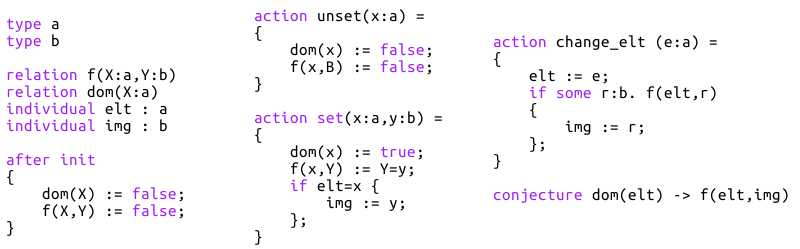
\includegraphics[width=15cm]{NonMonotonicExLarge}
    \\
    The keyword \textit{individual} is used to declare a variable, and the construction \textit{if some \(x\). \(\phi(x)\) \{ statement \}}
    assign to the variable \(x\) a value \(v\) such that \(\phi(v)\) is true and executes \textit{statement}. If no such value \(v\) exists,
    \textit{statement} is not executed.

    Basically, this example defines the following:
    \begin{itemize}
        \item Two uninterpreted sorts \(a\) and \(b\).
        \item A relation \(f\) from \(a\) to \(b\) that will represent a partial function, and \(dom\) its domain. It might look curious to not directly define a function instead,
        but it is sometimes useful for the decidability because functions are subject to stratification constraints.
        \item A variable \(elt\) in \(a\) and a variable \(img\) in \(b\). If \(elt\) is in the domain of \(f\), then \(b\) should always
        correspond to the image of \(elt\) by \(f\) (this specification is defined at the end with the keyword \textit{conjecture}).
        \item The init action, and some other actions to set/unset a value of \(f\) and to change the value of \(elt\).
    \end{itemize}

    This code satisfies the conjecture, however the conjecture is not inductive. Here is a counterexample:\\

    \begin{minipage}{0.45\textwidth}
        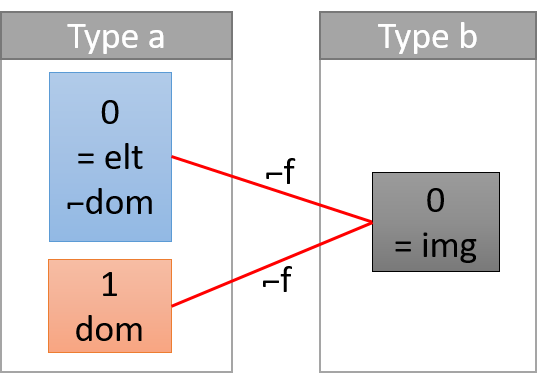
\includegraphics[width=8cm]{NonMonotonicExCounterexample}
    \end{minipage} \hfill
    \begin{minipage}{0.45\textwidth}
        Domain for \(a\): \(\{a_0,a_1\}\)\\
        Domain for \(b\): \(\{b_0\}\)\\
        Constraints on interpretations:\\
        \(elt = a_0\)\\
        \(\neg dom(a_0)\)\\
        \(dom(a_1)\)\\
        \(img = b_0\)\\
        \(\neg f(a_0,b_0)\)\\
        \(\neg f(a_1,b_0)\)\\
        Execution: change_elt(\(a_1\))
    \end{minipage}\\

    This state satisfies the conjecture because we have \(\neg dom(elt)\), but after executing change_elt(\(a_1\)) the conjecture will be broken.
    Applying the method described in the previous section will give the following invariant:
    \(\forall A:a. \neg(\neg dom(elt) \land dom(A) \land A \neq elt \land \neg f(elt,res) \land \neg f(A,res))\)

    However, this invariant is not correct: for instance, the following state doesn't satisfy it and can be obtained through a valid execution:

    \begin{minipage}{0.45\textwidth}
        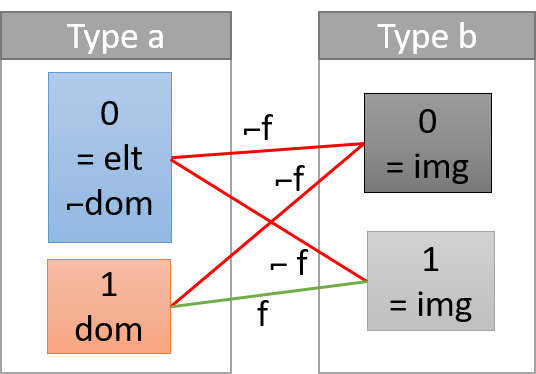
\includegraphics[width=8cm]{NonMonotonicExValid}
    \end{minipage} \hfill
    \begin{minipage}{0.45\textwidth}
        One element \(b_1\) has been added to \(b\)\\
        with the following new interpretations:\\
        \(\neg f(a_0,b_1)\)\\
        \(f(a_1,b_1)\)\\
        This time, the conjecture remains satisfied after executing any action.\\
        In particular, executing change_elt(\(a_1\)) will not break the conjecture anymore.
    \end{minipage}\\

    Indeed, the course of the execution of change_elt(\(a_1\)) can be changed just by adding a new element to \(b\)
    (without changing anything else). In this example, it is due to the use of the \textit{if some} statement.
    More generally, it can be caused by non-determinism, by the use of quantified formulas, or anything that explore all the elements of a type.

    \begin{definition}[Monotonicity]
        A statement \(s\) is monotonic iff, for any two states \(S_1\) and \(S_2\) such that \(S_1 \sqsubseteq S_2\)
        (\(S_1\) is a substructure of \(S_2\)), any states \(S_1'\) and \(S_2'\) that can respectively be obtained after executing
        \(s\) on \(S_1\) and \(S_2\) are such that \(S_1' \sqsubseteq S_2'\).

        An invariant \(P\) is monotonic iff, for any two states \(S_1\) and \(S_2\) such that \(S_1 \sqsubseteq S_2\),
        if \(S_1\) \textbf{doesn't} satisfy \(P\) then \(S_2\) doesn't satisfy \(P\) neither.
    \end{definition}

    \begin{property}
        The naive counterexample generalization method always generates correct invariants if the action involved is monotonic
        \textbf{and} the broken invariant is monotonic.
        Otherwise, it can generate incorrect invariants.
    \end{property}

    \section{A solution: symbolic bounded verification}

    The results of the naive counterexample generalization method can be improved by using symbolic bounded verification [REF].
    We says that a formula is a k-invariant if is satisfied by any execution starting from the init action and followed by at most k
    other actions. More formally, a formula \(Q\) is a k-invariant iff:

    \( A \Rightarrow \bigwedge\limits_{j=0}^k wp(\text{init}; (\text{action}_1|\ldots|\text{action}_n)^j, Q) \)\\
    where \(A\) refers to the axioms and `\(\text{statement}^j\)' represents the sequential composition of \(j\) copies of `statement'.

    According to section 1.4, checking the validity of this formula (for a given \(k\)) is decidable (for \(A\) of the form \(\exists^*\forall^*\) and \(Q\) of the form \(\forall^*\exists^*\)).

    This concept of k-invariant can improve the naive counterexample generalization in three points:
    \begin{itemize}
        \item It could allow us to know when a generated invariant is not correct.
        Actually, we cannot be sure that an invariant is correct using this method (because it is bounded to executions of length \(k\)),
        but in practice taking \(k=5\) is sufficient to detect incorrect invariants.
        \item It allows us to generate simpler and more general invariants. Indeed, instead of generating a formula that
        aggregates all constraints of the initial state of the counterexample, we are able to only keep a minimal number of constraints
        such that the resulting invariant is still correct. It can be done quite efficiently by computing an unSAT core using a SMT-solver.
        \item If the program that we want to check is not correct (it doesn't match the specification), symbolic bounded verification
        allows us to find it out, while a naive counterexample generalization would just generate incorrect invariants.
    \end{itemize}

    This method of counterexample generalization using symbolic bounded verification is the method currently implemented by IVy in order to
    help the user to synthesize inductive invariants interactively.\\

    \textbf{Correctness:} Can sometimes generate incorrect invariants, but most of times the symbolic bounded verification prevents it from
    happening (in this case, this method is not able to propose a new invariant).\\

    \textbf{Decidability:} All invariants generated are universal, so it never causes any decidability issue.\\

    \textbf{Simplicity:} Invariants generated are very simple. They are more focused than weakest preconditions
    (because they are issued from one precise counterexample) and do not contain any useless litteral.\\

    Almost all our criteria are fullfilled. However, it can sometimes generate incorrect invariants if the boundary \(k\) for
    symbolic verification is too low (sometimes we can't go beyond \(k=3\) in a reasonable time).
    Moreover, it can only generate universal invariants. Thus, in the case of non-monotonic counterexamples, it can fail to propose an invariant.

\chapter{My contributions}

    % First contribution: formalism and proofs above.

    \section{Filtering constraints using code analysis}

    % Complementary to symbolic bounded verification

    % Can also detect non-monotonicity! Give some inductive rules...

    \section{Case of non-monotonicity}

    \section{Weakening the conjecture}

    % Not always decidable!
    % Characterize it:
    % decidable when studied invariant is universal only,
    % axioms involved with mutation are existential only
    % assumption are existantial only

    \section{Guarantees}

\chapter{Conclusion}

    \section{Comparison of the different methods}

    % symbolic bounded verification generalized better than my method

    \section{What remains to be done}

    % Combine the two methods together (use symbolic bounded verification at the end to generalize, so we can have advantages of both methods)

    \section{Lessons from this internship}

%\chapter{Annexes}
    %\section{RML example: a leader election protocol}
    %\section{Comparison of results on different examples}

\bibliographystyle{unsrt}
\bibliography{sample}

\end{document}

